\begin{document}

Global climate change and the greenhouse effect is often a reocurring political subject. From 1722-2013, the Swedish Meteorological and Hydrological Institute (SMHI) collected daily temperature measurements from uppsala and the Stockholm region, Sweden. This data will be used to show the distribution of the yearly average temperature in this region from 1722-2013. Further more, analysis of this data will provide a moving average of the yearly average temperature. The moving average will be fitted with a $a(x-1840)\cdot cos(bx)$ function, trying to se if the future temperature is not only increasing, but actually oscillating with an increasing amplitude, correlated to the human development since the industrial revolution in 1840~\cite{industrial}.

\subsection{Method}
There are two versions of this code, \texttt{tempExtrap.cpp}. One analyzes all data from 1723-2013 in the Stockholm region, found in the \texttt{master} branch of the git repository. One analyzes only data taken in uppsala, found in the \texttt{ref} branch on the repository.

Dailytemperatures were read from raw data and put into a multi dimensional vector according to the \texttt{readData} or \texttt{readAllData} function. After this was called from \texttt{tempEx} a simple for loop converted this into a 2-D data vector containing year and temperature, with one entry for each day.

The next step was to calculate the yearly averages from the data. For the uppsala only data, this was done by \texttt{averages1} in the \texttt{ref} branch. This iterated through all the elements of the data vector. If the year of the current element was not larger than the previous, then the temperature of the current element was added to a temperature sum and the number of days counted so far was incremented. When the current year became larger than the previous, the previous year was pushed into a dummy vector along with the average temperature. This dummy vector was then pushed into another vector, creating a 2D averages vector containing one element per year with that year's average temperature.

For the data in the whole Stockholm region, using \texttt{averages} in the \texttt{master} branch, the first year, 1722, was skipped because its measurement started after the 1st of January. After 1722 the data vector was iterated in steps of the years with two nested for loops. In the outer loop, if the year was a leap year, an inner for loop iterated from day 1 to 366 and pushed the average temperature and the year into a dummy vector then into an averages vector. Similarly if the year was not a leap year, it was then iterated 365 times and the average was calculated appropriately.

With the data of yearly averages at hand, it was processed for plotting. To do this, the total average temeperature from all the yearly average temperatures was calculated. With a for loop iterating through the data elements and simple if statements, the average temperatures and corresponding year were pushed into one vector containing all temperatures above the total average, and one vector containing those below. These two new vectors are not used for further analysis, but purely used for plotting.

The average temperature vector was then used to calculate a moving average. The goal of this moving average is to take the yearly averages in groups and take the average yearly temperature for that group. This will make the fluctuations in the data less extreme and make it easier to fit. Similarly to the other average calculation functions, this iterated through the average vector and for each element added its temperature to a sum. If the iteration counter was the size of the desired group size, then the average of the average temperatures was pushed into a vector for the y-values. For the x-values, the current year, corresponded to the initial year, plus the number of groups so far times the group size. Plus half a group size inorder to represent the middle of the group. If the number of years is not divisible by the group size then the last years will not be represented. This is accomodated for, outside the for loop, the latest value for the sum i and the latest number of years so far are pushed as an average into the y-vector. An appropriate value is also pushed to the x-vector.

These moving average y- and x-values, using a group size of 30, were then put into a \texttt{TGraph} object, and a fit function was added to this graf. The function was of the form $A*(x-1840)*cos(B*x))$, where A and B are parameters. The graph and the fit were then plotted together with the above and belov vectors, as bar graphs, mentioned earlier. A second moving average was also added with a group size of 10.

The main function \texttt{tempEx} then returned the value of the fit function evaluated at the desired year specified in \texttt{project.cpp}.

\subsection{Results and Conclusion}

\begin{figure}[ht]
\begin{center}
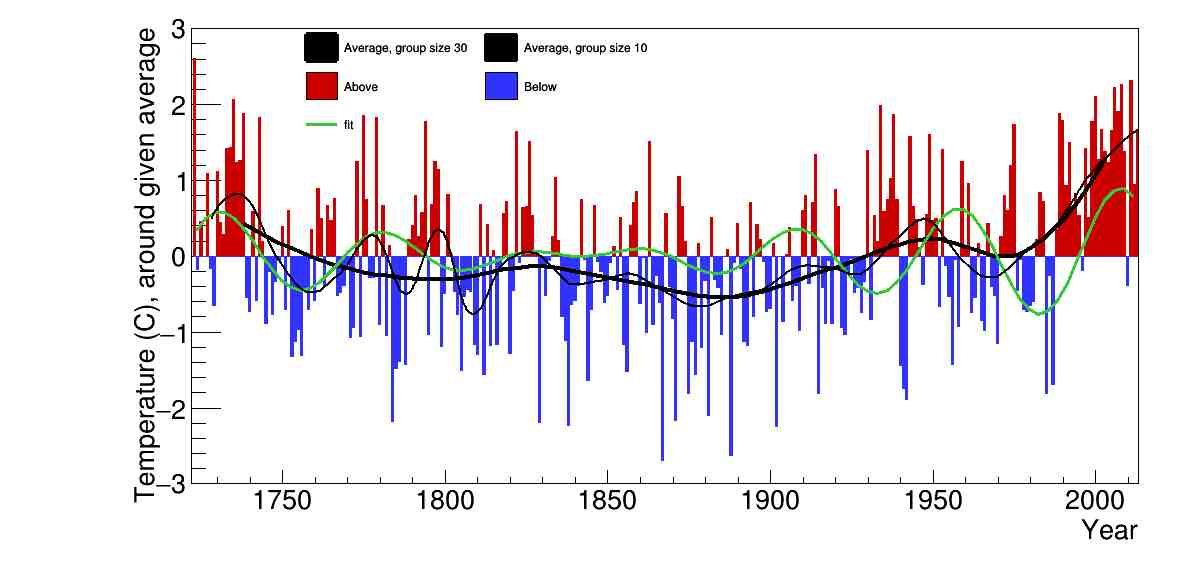
\includegraphics[scale=0.35]{extrapolatedDataFit.jpg}
\caption{\label{fig:extrap1}Shows the yearly average temperature around an average of 5.9 $^{\circ}$C from data taken in the Stockholm region form 1723-2013. The thick and thin black lines show moving averages with a grouping size of 30 and 10 respectively. The green fit is of the form $A*(x-1840)*cos(B*x))$}
\end{center}
\end{figure}

\begin{figure}[ht]
\begin{center}
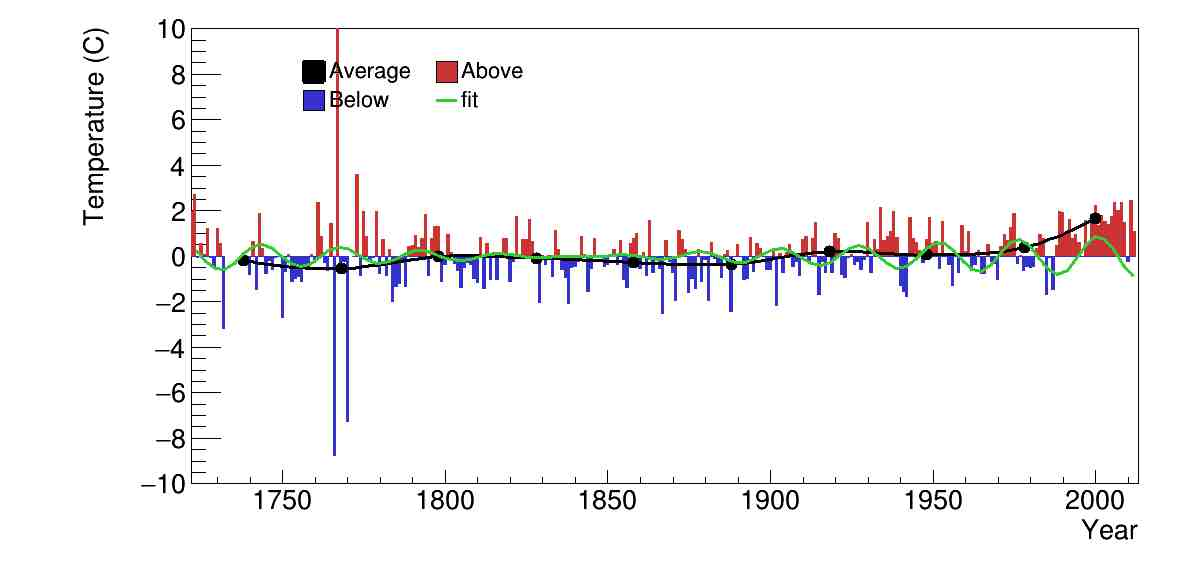
\includegraphics[scale=0.35]{notleap.jpg}
\caption{\label{fig:extrap2}Shows the yearly average temperature around an average of 5.9 $^{\circ}$C from data taken only in uppsala 1722-2013. This does not consist of data taken daily. The thick and thin black lines show moving averages with a grouping size of 30 and 10 respectively. The green fit is of the form $A*(x-1840)*cos(B*x))$}
\end{center}
\end{figure}

Figure \ref{fig:extrap2} shows the data plotted as described for only measurements in uppsala. Figure \ref{fig:extrap1} shows the data plotted as described for the whole Stockholm region. When comparing these two, it can be seen that strictly using data from one location can really affect the results since not every day of the year is recorded. For example, at the warmest peak in 1776, only 20 data points came from the uppsala station consecutively in the month of June. Which definately skews the data. Because of this, we perform our analysis on the data from the whole Stockholm region. The results in Figure \ref{fig:extrap1} show a periodically oscillating average yearly temperature around 5.9 $^{\circ}$C. The best fit was determined to be $0.005(x-1840)cos(0.125x)$. This achieves a $\chi ^2=1.2$, which is surprisingly good for such a simplistic model. Extrapolating with this function gives an average temperature of 5.88 $^{\circ}$C year 2050. 

In conclusion, the yearly temperatures do in fact oscillate over time. However, it is clearly seen in the data that the more recent years have been concistently warmer and a more proper model, using global data could most likely show proof of global warming. It is interesting to see that such a simple model as ours does make a good fit with the data. It is also interesting that a temperature increase, such as the one seen in the end of Figure \ref{fig:extrap1},\ref{fig:extrap2}, is visible in data just obtained in the Stockholm region.





\end{document}